\chapter{Obfuscators in Android Malware}

In this experiment we use different obfuscators to modify parts of an android malware. By systematically obfuscating different parts of the code, we can gain insight into the parts which contribute most to the detection of malware. Once we have this information, we can then determine efficient ways to make the malware detectors more robust and be less resilient to code obfuscators.

\section{Experiment}
For this project, we use a tool called AAMO (Another Android Malware Obfuscator) \cite{aamo}. This tool gives us various obfuscators for use with our experimentations. The obfuscators can be used independently or in combination with other obfuscators to increase their effectiveness. Using this tool, we decompile a android file, perform obfuscation operations on them, and recompile the file again. In this experiment, we use the source code provided by the developers of AAMO \cite{aamo} and available at \cite{gitLoc}. This tool forms the basis of the work presented in this thesis.

The steps involved in this are detailed below:
 
 \begin{enumerate}
	 \item Obtain an APK file.
	 \item Decompile the APK file into Smali.
	 \item Get the list of obfuscators passed into the program.
	 \item Apply the obfuscators one after the other on the decompiled apk file.
	 \item Repackage the decompiled file into an APK.
	 \item Sign the APK file to maintain its integrity.
 \end{enumerate}
 
 Performing the above steps ensures that the apk file is not corrupted and its usage is not affected. We perform this to make it difficult for a malware detector to detect the apk file as a malicious one. The entire flow of the experiment is depicted in Fig. \ref{procedure}.
 
  \vspace{3mm}
  \begin{center}
  	%\centering
  	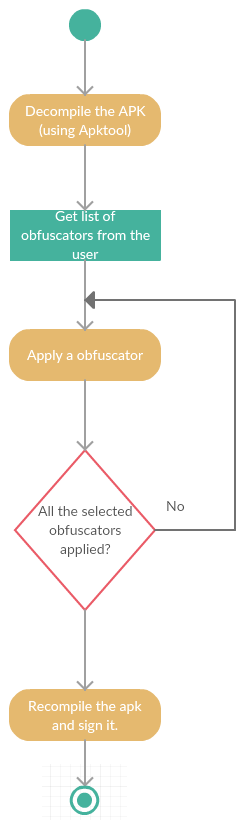
\includegraphics[width=50mm]{procedure.png}
  	\captionof{figure}{Experiment flow}
  	\label{procedure}
  \end{center}
  \vspace{3mm}
  
 As shown in Fig.\ref{procedure}, the final encryption would let the malicious file be signed with a valid signature and thus eliminating any traces of the apk file having been compromised.
 
\subsection{Uses of the obfuscator}

Using the obfuscator in this step has various advantages for our experiment. One of the primary uses is to make the job of the malware detector more difficult. Since most of the malware detectors do not take into account polymorphic and oligomorphic malware, using obfuscators will let us know which parts of a malware factor into the detection score computed by individual detectors. In this experiment, we use the following 14 obfuscators to test out the resilience of the malware detectors:

\begin{enumerate}
	 \item  Resigned
	 \item  Alignment
	 \item  Rebuild
	 \item  Fields
	 \item  Debug
	 \item  Indirections
	 \item  Renaming
	 \item  Reordering
	 \item  Goto
	 \item  Arithmetic Branch
	 \item  Nop
	 \item  Lib
	 \item  Manifest
	 \item  Reflection
\end{enumerate}

These obfuscators enable us to test the various aspects of a apk file and help us determine the ones that are really useful to a malware detector. When a particular obfuscator is run, it runs a function that is specific to that particular obfuscator and applies that function to all the parameters that match the criteria for that specific obfuscator.

Each of the obfuscator is discussed here in detail. 

\subsubsection{Resigned}

This obfuscator decompiles an apk and just resigns the apk file after compilation. Not much change is done to the application file in itself. The purpose of this obfuscator is to attempt defeating malware detectors that try to use signatures of certain known malware sources to classify a malicious file.

\subsection{Alignment}

This obfuscator makes use of the zipalign utility of android. Zipalign is a tool that is used to provide optimization techniques to APK files. The tool causes all uncompressed data within the APK to start with a particular alignment relative to the file's beginning. The Alignment obfuscator changes this alignment before recompiling the apk file.

\subsection{Rebuild}
This obfuscator rebuilds the application file without performing any changes. The unpacking and repackaging of the apk file affects the timestamp, signature of the apk and other factors that help in identifying the origin of the file. Some smart malware detectors are able to detect these changes and do not let the file pass through it.

\subsection{Fields}
This is a relatively simple obfuscator that just renames the fields that are used in the application. This is done after the decompilation of the apk file. The smali is analyzed for locating the fields that are used in the source code and these are renamed.

\subsection{Debug}
The debug obfuscator removes all information related to debug from the files. This is performed not only on the smali file, but throughout the source code as well. Without the debug information, the APK file becomes slightly different from the original file. Removal of the debug information also alters the size of the file and makes it different.

\subsection{Indirections}
Call indirections is an advanced obfuscation method in which various function calls are directed through different values. The obfuscator performs operations such as changing the register count, changing a method call and also redirecting all calls to the methods. This obfuscation completely changes the control flow of an application and makes it difficult to detect using a comparison model in dynamic analysis as well.

\subsection{Renaming}
All the variables in the sourcecode are renamed to different values. This is exactly like using substitutions to hide the original values. Renaming is also advantageous when certain signature and pattern matches are based on the names of the variables and functions.


\subsection{Reordering}
Using reordering will let us change the order of the code in the application. The obfuscator changes the location of certain parts of the code and adjusts the calls to it accordingly.  This makes it possible to evade signature based detection methods if the signature is based on the order of instructions or if it is based on the DEX opcodes.

\subsection{Goto}
In order to modify the control-flow structure of the application, forward and backward jumps are inserted into the code. These unconditional jump statements will be executed irrespective of how the program is run. This widely alters the flow and will make it very difficult to detect using conventional methods.

\subsection{Arithmetic Branch}
A constant value, known to the obfuscator, is used to achieve this obfuscation. This constant value is not known to the compiler. Using this constant value, the obfuscator is able to control the flow of execution of the program. The compiler assumes that either of the branches could be possible as the value for deciding the flow of control is not known. This is applied to methods with more than 2 parameters.

\subsection{Nop}
This is a classical and an easy way to obfuscate a program. In this, a "no-operation instruction" (known as a "NOP") is inserted into the source code. The number of such instructions inserted is randomized. These are inserted into methods to make them bloated and delay the execution time.

\subsection{Lib}
MD5 hashing is used to rename the file and path names.  A proxy method is created and used to handle the decryption of the values, when it is required by the system.


\subsection{Manifest}
The AndroidManifest.xml file is modified by this obfuscator. The manifest file contains important information related to the application's usage and permissions. This obfuscator opens up the file and encrypts the values for the resources and also replaces the characters in user defined identifiers.

\subsection{Reflection}
This obfuscator acts similar to the code reodering obfuscator. The reflection obfuscator takes advantage of the Android dynamic code loading API. All the static method calls are converted into reflection calls and the the reflect method is invoked on a string that contains the target method's name.